
\documentclass[10pt,a4paper]{article}
\usepackage[utf8]{inputenc}
\usepackage[french]{babel}
\usepackage{listings}
\usepackage{graphicx}
\usepackage[left=2cm,right=2cm,top=2cm,bottom=2cm]{geometry}
\usepackage{hyperref}
%opening
\title{TP1 Mesures simples de tensions}
\author{Nicolas Vadkerti}
\usepackage{listings} % Required for inserting code snippets
\usepackage[usenames,dvipsnames]{color} % Required for specifying custom colors and referring to colors by name

\definecolor{DarkGreen}{rgb}{0.0,0.4,0.0} % Comment color
\definecolor{highlight}{RGB}{255,251,204} % Code highlight color

\lstdefinestyle{Style1}{ % Define a style for your code snippet, multiple definitions can be made if, for example, you wish to insert multiple code snippets using different programming languages into one document
language=Perl, % Detects keywords, comments, strings, functions, etc for the language specified
backgroundcolor=\color{highlight}, % Set the background color for the snippet - useful for highlighting
basicstyle=\footnotesize\ttfamily, % The default font size and style of the code
breakatwhitespace=false, % If true, only allows line breaks at white space
breaklines=true, % Automatic line breaking (prevents code from protruding outside the box)
captionpos=b, % Sets the caption position: b for bottom; t for top
commentstyle=\usefont{T1}{pcr}{m}{sl}\color{DarkGreen}, % Style of comments within the code - dark green courier font
deletekeywords={}, % If you want to delete any keywords from the current language separate them by commas
%escapeinside={\%}, % This allows you to escape to LaTeX using the character in the bracket
firstnumber=1, % Line numbers begin at line 1
frame=single, % Frame around the code box, value can be: none, leftline, topline, bottomline, lines, single, shadowbox
frameround=tttt, % Rounds the corners of the frame for the top left, top right, bottom left and bottom right positions
keywordstyle=\color{Blue}\bf, % Functions are bold and blue
morekeywords={}, % Add any functions no included by default here separated by commas
numbers=left, % Location of line numbers, can take the values of: none, left, right
numbersep=10pt, % Distance of line numbers from the code box
numberstyle=\tiny\color{Gray}, % Style used for line numbers
rulecolor=\color{black}, % Frame border color
showstringspaces=false, % Don't put marks in string spaces
showtabs=false, % Display tabs in the code as lines
stepnumber=5, % The step distance between line numbers, i.e. how often will lines be numbered
stringstyle=\color{Purple}, % Strings are purple
tabsize=2
}

\newcommand{\insertcode}[2]{\begin{itemize}\item[]\lstinputlisting[caption=#2,label=#1,style=Style1]{#1}\end{itemize}} 


% \insertcode{"Scripts/example.pl"}{Nena would be proud.} 

\begin{document}

\maketitle


\url{https://github.com/SlaynPool/TP1_SIGNAUX_ET_INTERFACAGE/}
\section{Mise en oeuvre de la carte Arduino}
Pour cette partie, j'ai realiser le montage prévu dans le tp :
\begin{figure}[h!]
\centering
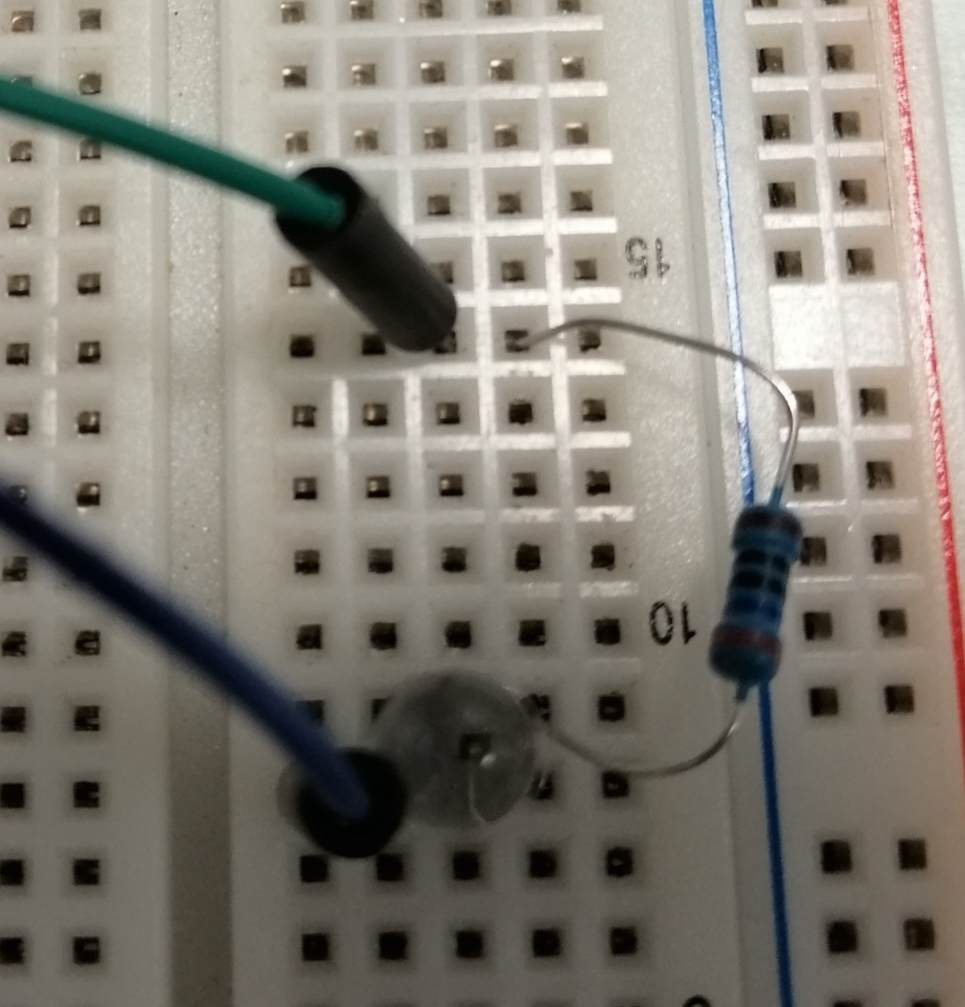
\includegraphics[scale=0.20]{screen/1.jpg}
\caption{Montage}
\label{fig:net }
\end{figure}
Le fils rouge est connecté sur le PIN 13 de mon ESP, et le fils vert sur le GND.
Voici donc le code 
\insertcode{code/blink.txt}{Code 1}
Ma led Clignotte correctement.\newpage
\section{Analyse du convertiseur CAN}
\subsection{Détérminer l'expression de V1, puis celle de la tension Vi dans le cas général.}
Nous avons :\\
R= 330 Ohms\\
U= 3.3 V\\
V1= (330/(5*330))*3.3=0.66V\\
L'expresion de Vi est donc:
Vi: (R/(iR)*330
\subsection{mise en place du montage}
\begin{figure}[h!]
\centering
\includegraphics[scale=0.10]{screen/2.jpg}
\caption{Montage}
\label{fig:net }
\end{figure}
\subsection{Tension mesuré}
\begin{tabular}{|l|l|l|}
\hline
    Resistance & Valeurs Theorique (V) & Valeurs Mesures (V)\\ \hline
    1 & 0,66 & 0,657\\ \hline
    2 & 0,82 & 1,31\\ \hline
    3 & 1,1 & 1,97\\ \hline
    4 & 1,65 & 2,64\\ \hline
    5 & 3,3 & 3,31\\ \hline
    
\hline
\end{tabular}
\subsection{AnalogReadSerial}
On branche donc un fils sur le port noté VP de notre stm32. On modifie notre vitesse pour le port serie. Voici le resultat de mon moniteur Serie si je branche mon fils après la dernier resistance :
\begin{figure}[h!]
\centering
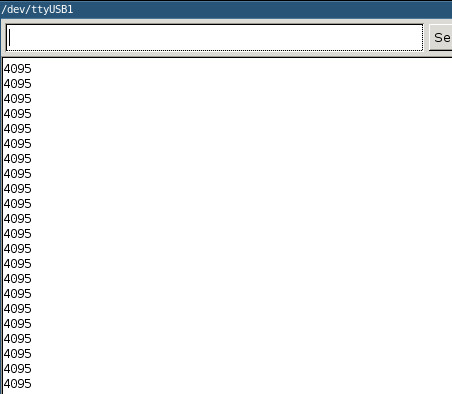
\includegraphics[scale=0.50]{screen/3.jpg}
\caption{Moniteur Serie}
\label{fig:net }
\end{figure}

La ligne ``int sensorValue = AnalogRead(A0);'' sert à lire une tension sur un pin, ici le pin A0, puis la convertir en une valeur numerique à l'aide d'un CAN.
La fonction AnalogRead() renvoi donc un entier qui sera donc disponible dans la variable sensorValue.
\subsection{Resolution, plage de conversion, et pas de quantification}
valeur de N0= 0\\
valeur de N5 = 4095\\
On peut donc en déduire la Resolution du Convertiseur :\\
3.3/4095 = 0.000805, cela signifie que pour chaques n*0.000805 V une valeurs numerique est associée \\

La plage de conversion est donc de 0 à 4095 \\
\subsection{Pour l'ESP32, A0 est une entrée ou une sortie}
Pour l'ESP32, A0 est une entrée dans le sens qu'il lit des valeurs sur le pin

\subsection{Effectuer la lecture de N1}
On lit des valeurs entre 1468 et 1472 donc on a un ecart de 4 valeurs, et une Vmoyen de 1470. Si on converti cette valeur en Volt, on obtient donc 1470*0,000805= 1,183 V\\
\subsection{Effectuer toutes les lectures}
\begin{tabular}{|l|l|l|l|l|l|}
\hline
    Resistance & Valeurs Theorique (V) & Valeurs Mesures (V) & Ecart & Moyenne & V mesuré CAN \\ \hline
    1 & 0,66 & 0,657 & 4 & 632 & 0,50876 \\ \hline
    2 & 0,82 & 1,31 & 4 & 1470 & 1,183\\ \hline
    3 & 1,1 & 1,97 & 4 & 2305 & 1,855\\ \hline
    4 & 1,65 & 2,64 & 4 & 3169 &  2,551\\ \hline
    5 & 3,3 & 3,31 & 0 & 4095  &  3,296\\ \hline
    
\hline
\end{tabular}



\end{document}
